\documentclass[11pt, a4paper]{article}


%% Babel provides support for languages.  'english' uses British
%% English hyphenation and text snippets like "Figure" and
%% "Theorem". Use the option 'ngerman' if your document is in German.
%% Use 'american' for American English.  Note that if you change this,
%% the next LaTeX run may show spurious errors.  Simply run it again.
%% If they persist, remove the .aux file and try again.
\usepackage[english]{babel}

%% Input encoding 'utf8'. In some cases you might need 'utf8x' for
%% extra symbols. Not all editors, especially on Windows, are UTF-8
%% capable, so you may want to use 'latin1' instead.
% \usepackage[utf8]{inputenc}

%% The AMS-LaTeX extensions for mathematical typesetting.  Do not
%% remove.
\usepackage{amsmath,amssymb,amsfonts,mathrsfs}

%% LaTeX' own graphics handling
\usepackage{graphicx}
\graphicspath{ {./images/} }

\usepackage{array}
\usepackage{makecell}
\usepackage{hyperref}

%Change margins
\usepackage[left=1.5cm, right=1.5cm]{geometry}

\title{DRL Seminar Projekt Alain Keller}

\author{Alain Keller}
\begin{document}
\maketitle
\section{Problem}
The goal of this project was to train the ant from the Farama Gymnasium\footnote{\url{https://gymnasium.farama.org/environments/mujoco/ant/}} to move forward in one direction.
The current environment features a 8-dimensional action space with actions $a_1 \in [-1,1]$ and 
a 27-dimensional observation space with $o_i \in (-\infty, \infty)$.
The reward for each action is provided by the environment and cosnists of three parts.
The first reward is provided every step if the ant is still alive, the second is given every n steps and 
rewards when the ant moved forward in the x direction and the third is the squared action vector length to penalize large movements.
The rewards are weighted and summed to give a final reward.

Since the action space space is continous a classic Q-Learning approach is not suitable for this problem.

Therefore deep reinforcement learning methods were used to solve this problem.
As a first approach the REINFORCE \cite{REINFORCE} was used.
Later on the more modern Soft Actor Critic (SAC) \cite{haarnoja2018soft} was used.
\section{REINFORCE}
The implementation of the REINFORCE Agent is in the \textit{reinforce.py} file.
To first test the agent, it was used to solve a simpler problem, the Inverted Pendulum\footnote{\url{https://gymnasium.farama.org/environments/mujoco/inverted_pendulum/}}.
To enforce the agent to explore new actions, an $\epsilon$-greedy strategy was implemented to choose
the new action. It can be parmaetrized with a starting $\epsilon$, decay weight and a minimum $\epsilon$.
Every 10 iterations the current model is evaluated by running the model only with actions suggested by the trained policy.
To speed up the developement, the training routine was stopped, when a perfect scrore was achieved in the evaluation.
In Figures \ref{REIN:Pen_eval} and \ref{REIN:Pen_tra} the curves of the evaluation and train reward are depicted.
The agent sucessfuly trained a policy to balance the pendulum. This policy can be seen in the video in TODO

\begin{figure}
    \centering
    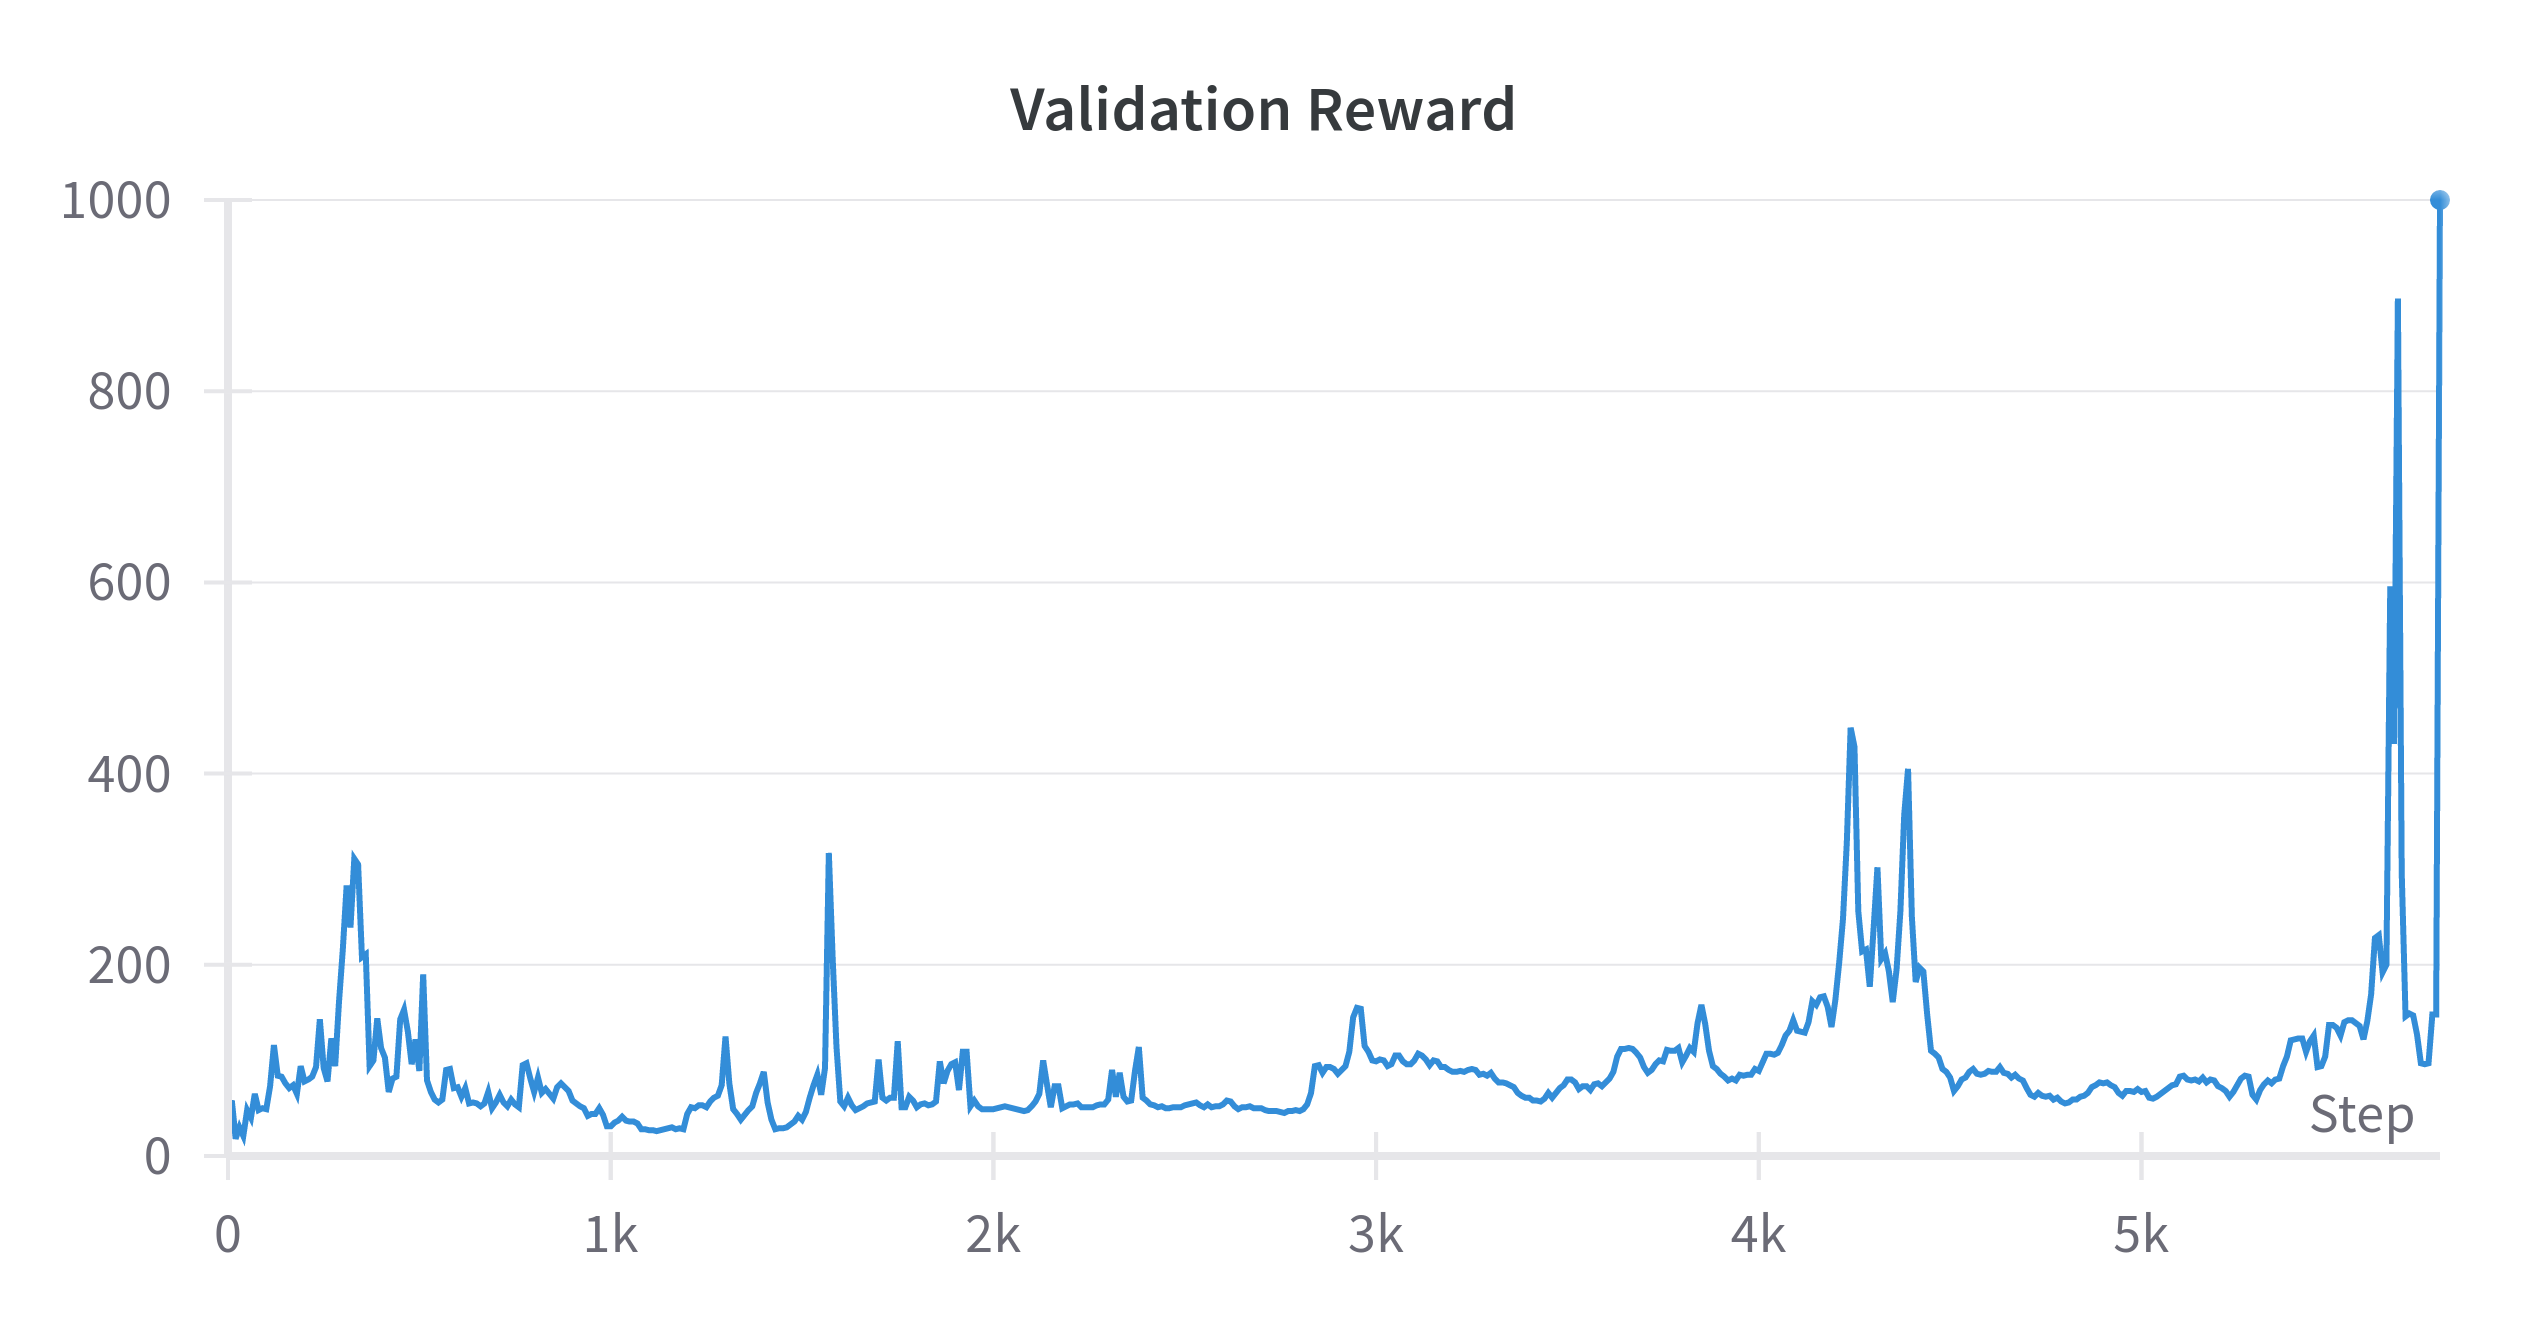
\includegraphics[width=13cm]{pendulum_eval.png}
    \caption{Evaluation run rewards vor the inverted pendulum environment}
    \label{REIN:Pen_eval}
\end{figure}

\begin{figure}
    \centering
    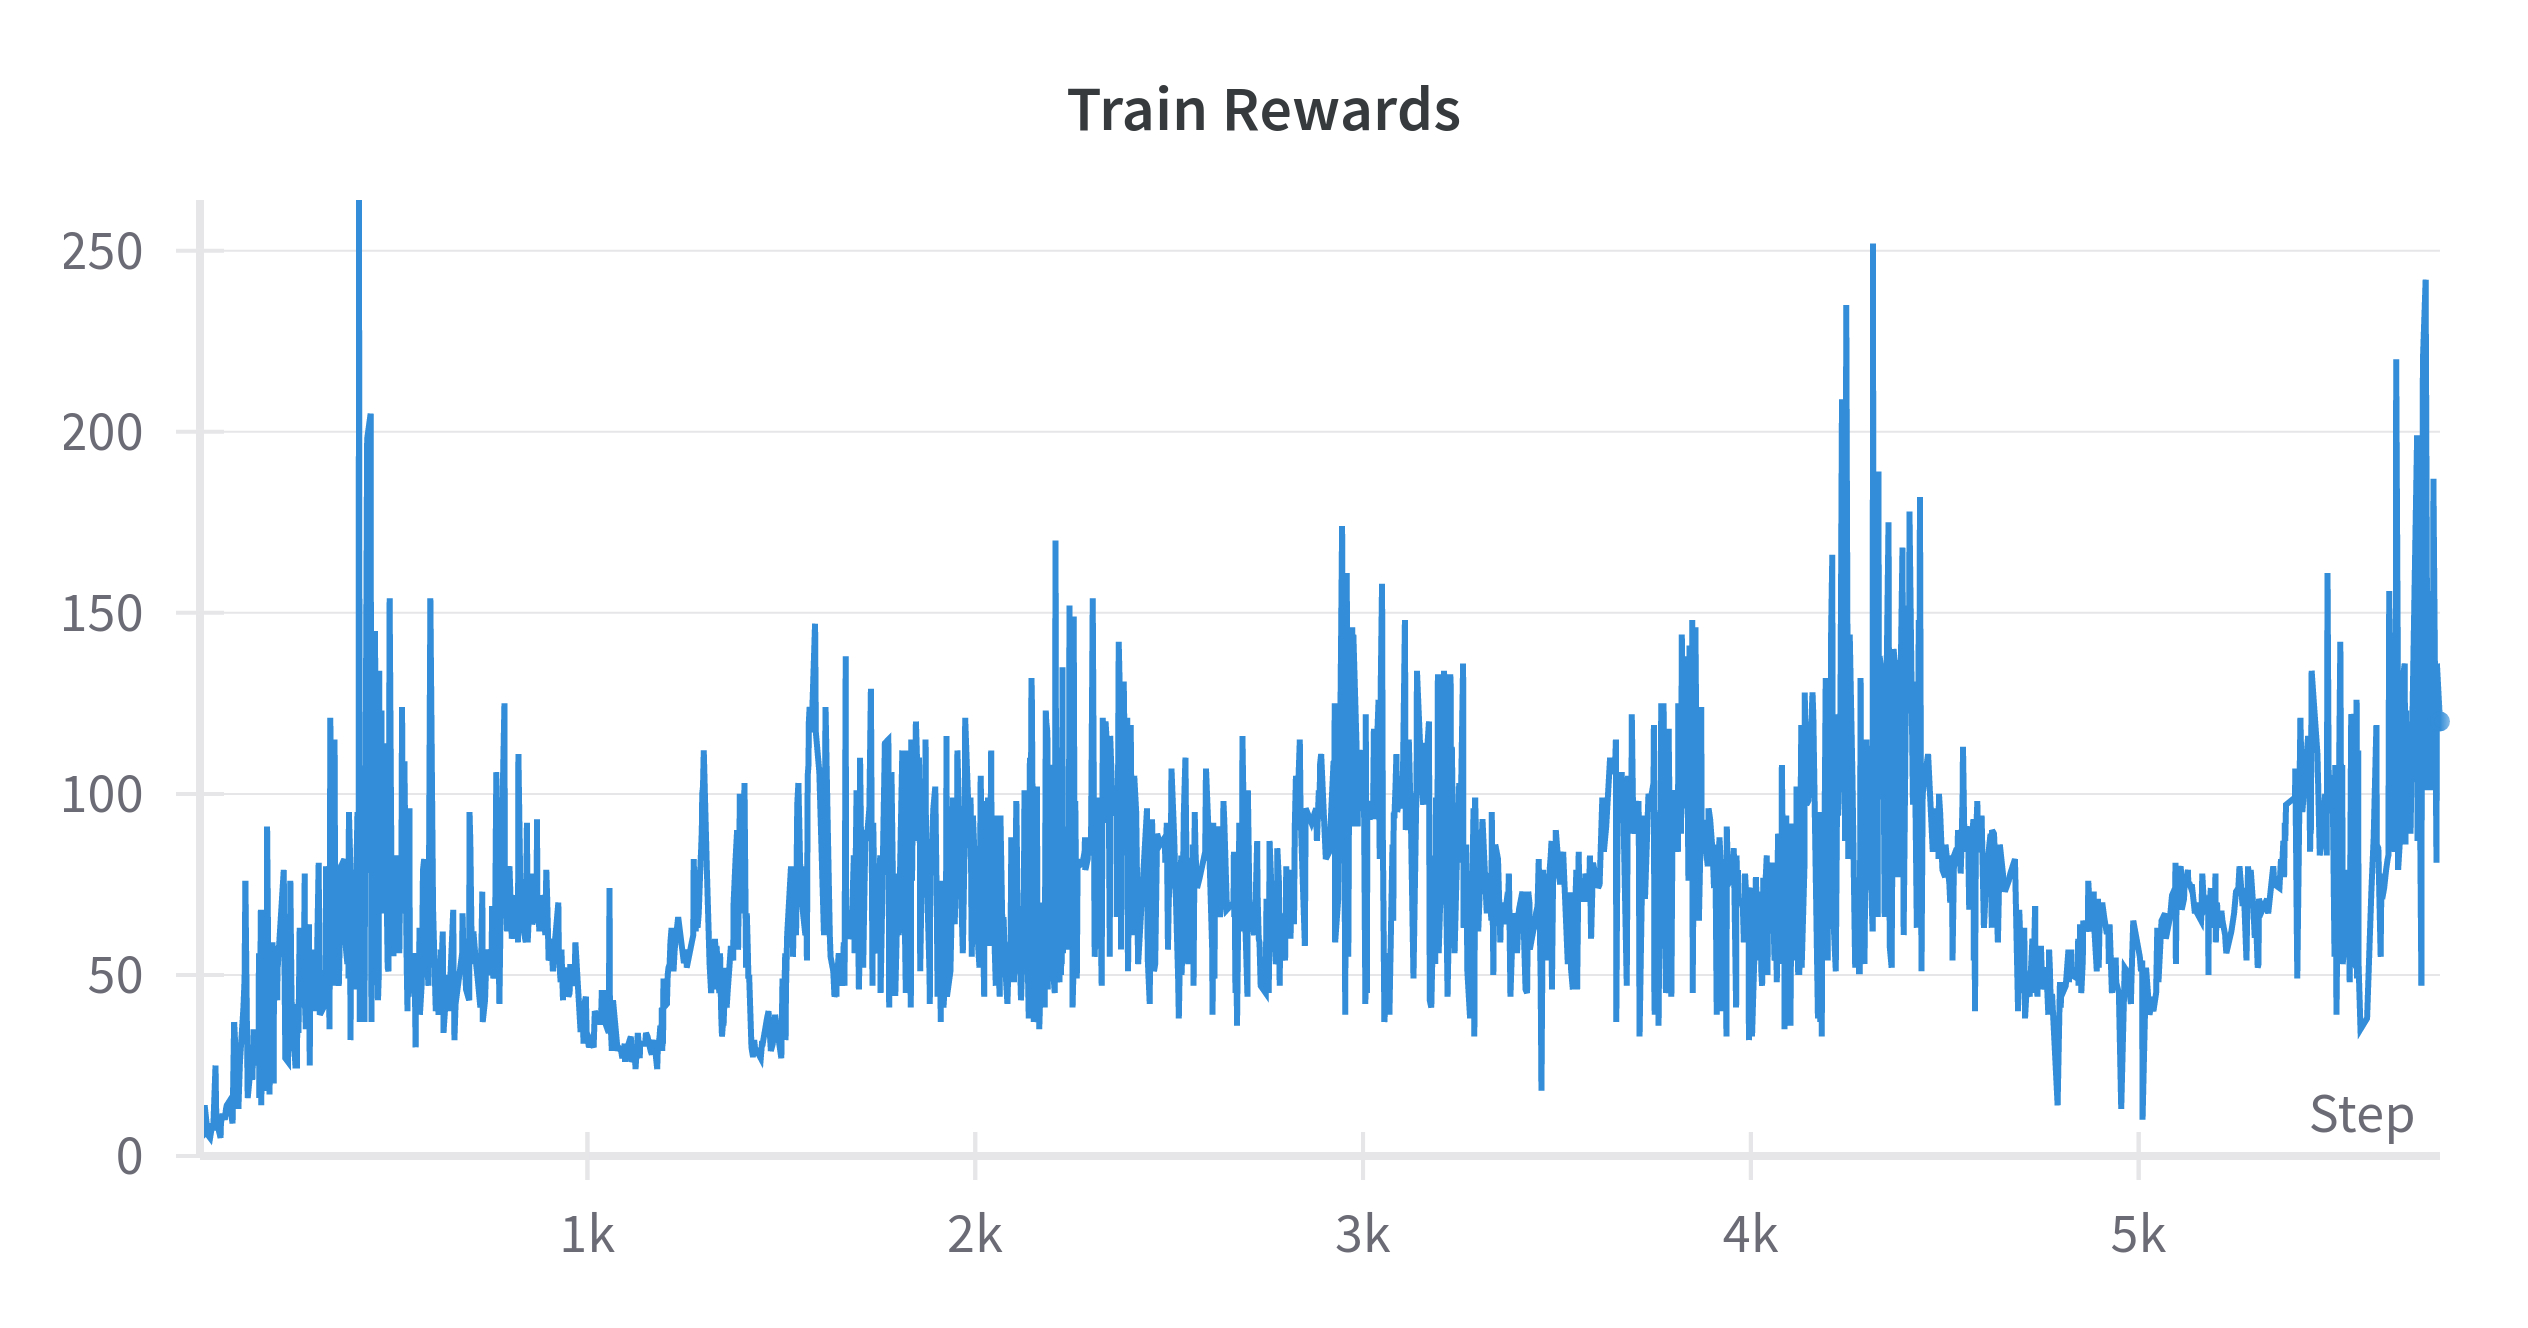
\includegraphics[width=13cm]{pendulum_train.png}
    \caption{Training run rewards vor the inverted pendulum environment}
    \label{REIN:Pen_tra}
\end{figure}

Showing that the implemented agent is able to learn the goal was to use it to train a policy
for the Ant environment.
This step turned out to be more challenging than anticipated.
With the environemnt being more complex it was expected, that more training would be
needed to achieve good results.
Within the given time frame the best result was a standing ant.
Figures \ref{REIN:ant_eval} and \ref{REIN:ant_eval} show the corresponding learning curevs.
The depicted training took around 18 hours.
The probelm that the ant did not learn to move forward lies probably in the hyperparameters like the
$\epsilon$ needed to explore. Additionally the REINFORCE actor may not be a well suited actor to
train the ant due to its simplicity.
\begin{figure}
    \centering
    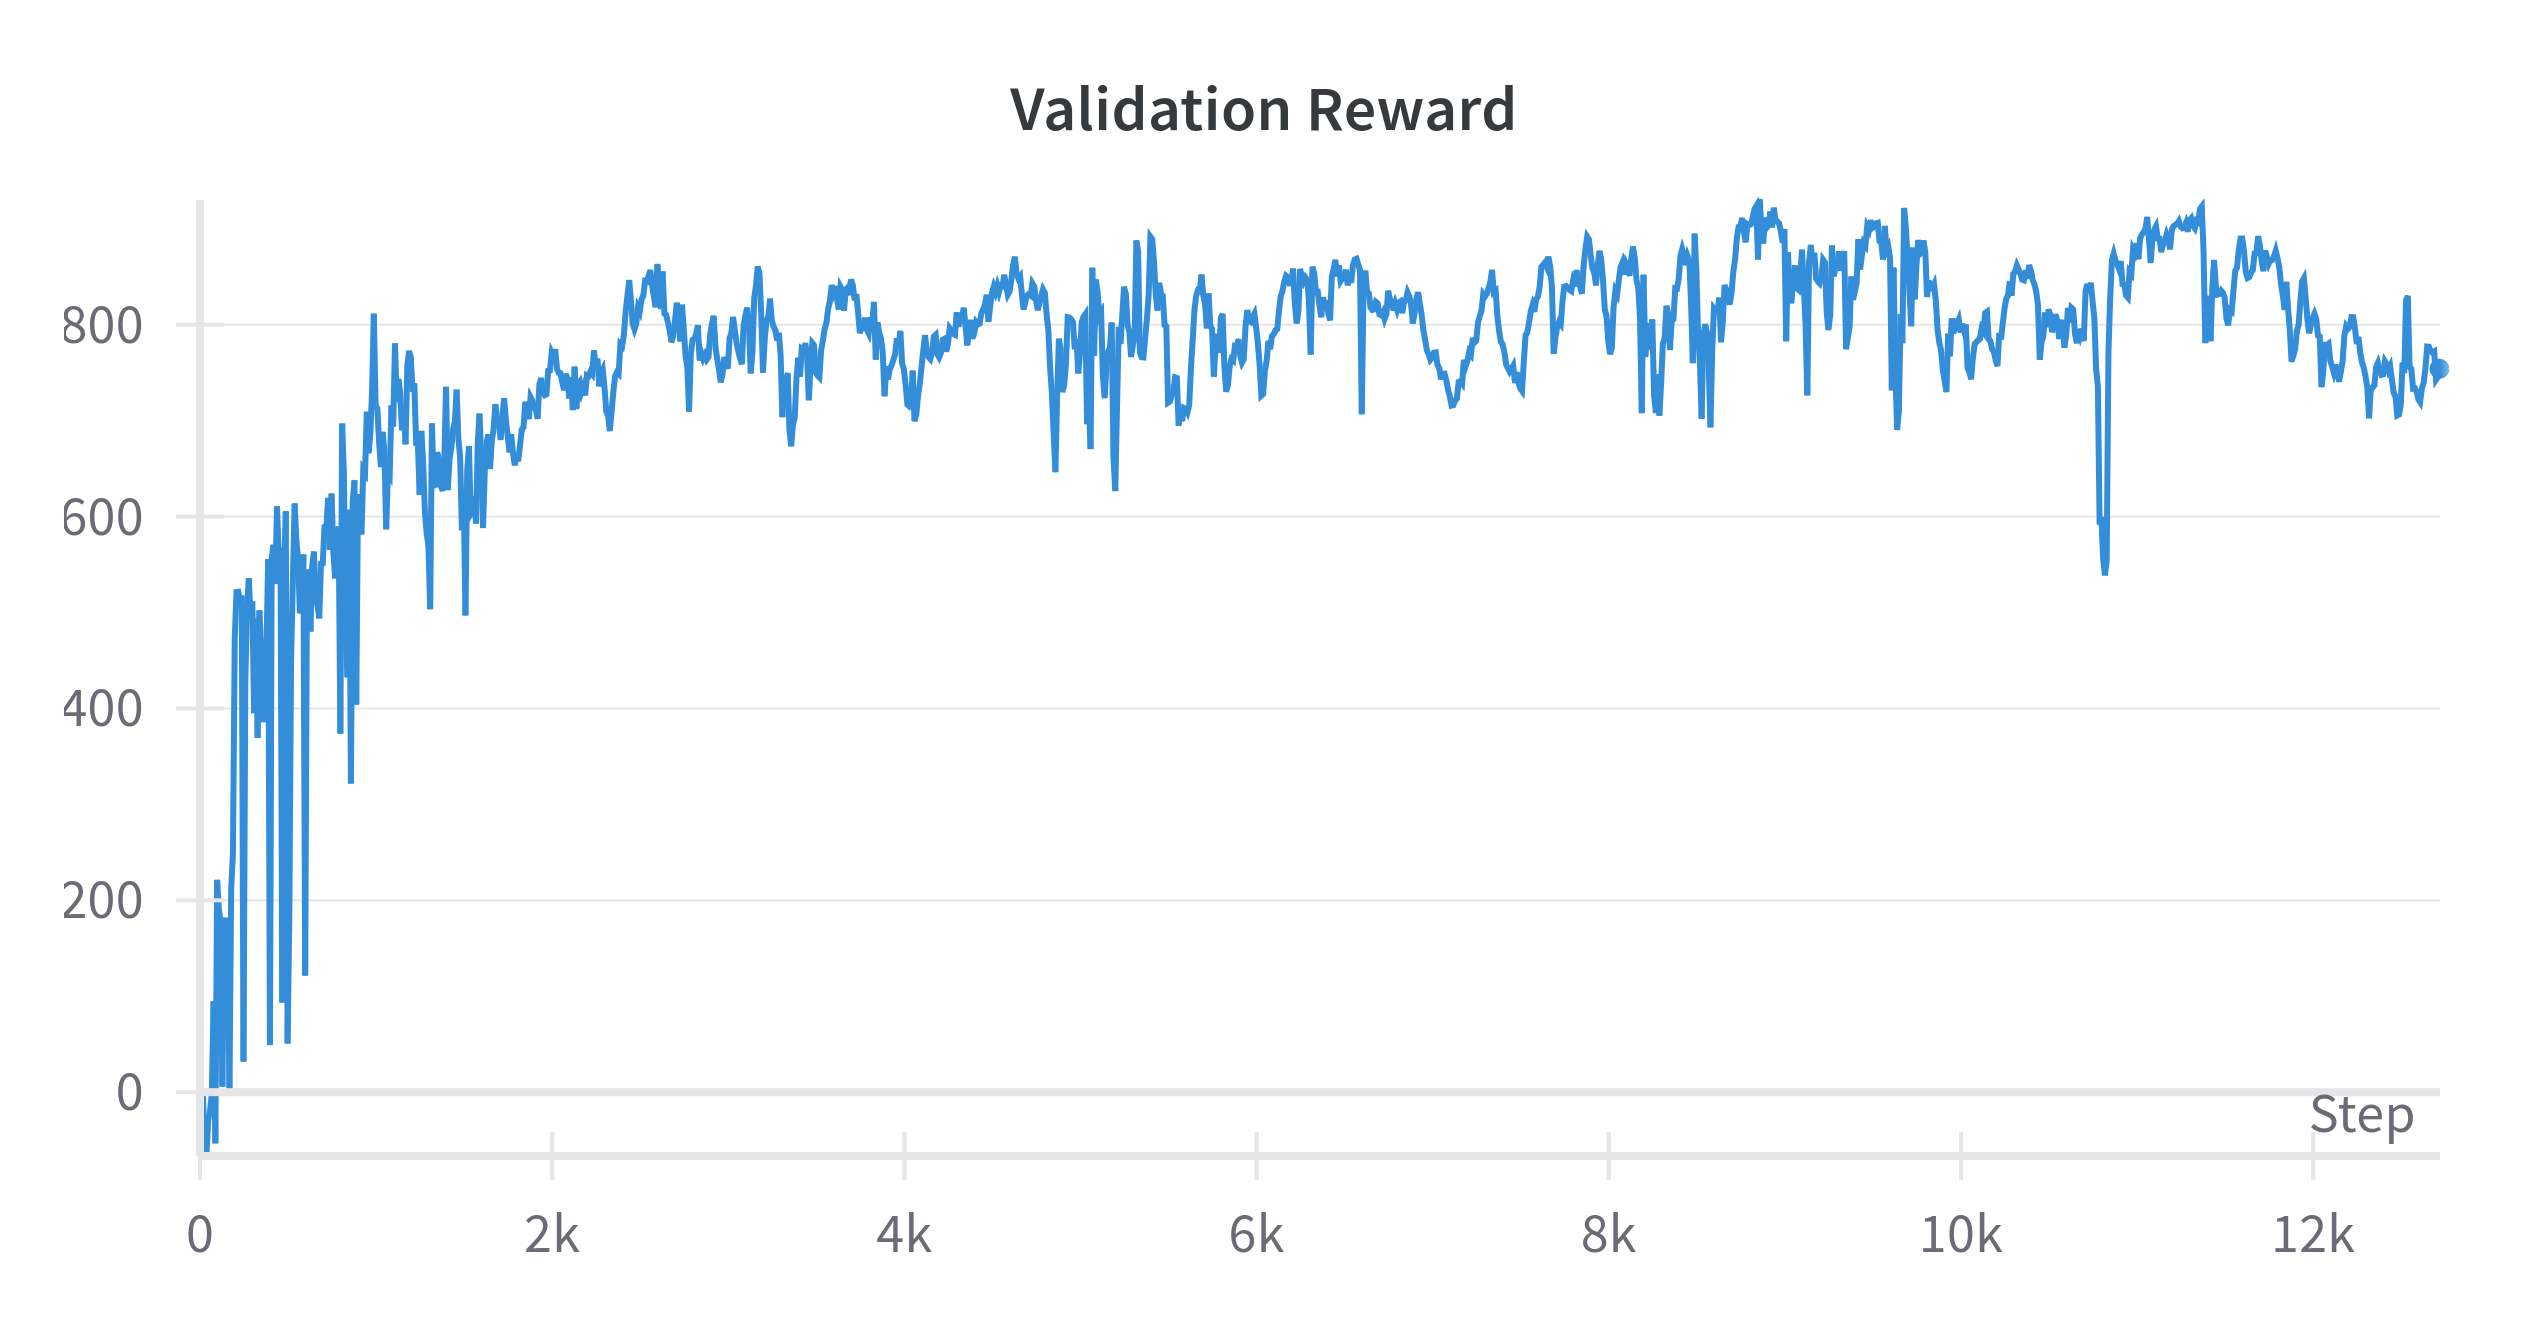
\includegraphics[width=13cm]{reinforce_ant_val.png}
    \caption{Evaluation run rewards vor the ant environment}
    \label{REIN:ant_eval}
\end{figure}

\begin{figure}
    \centering
    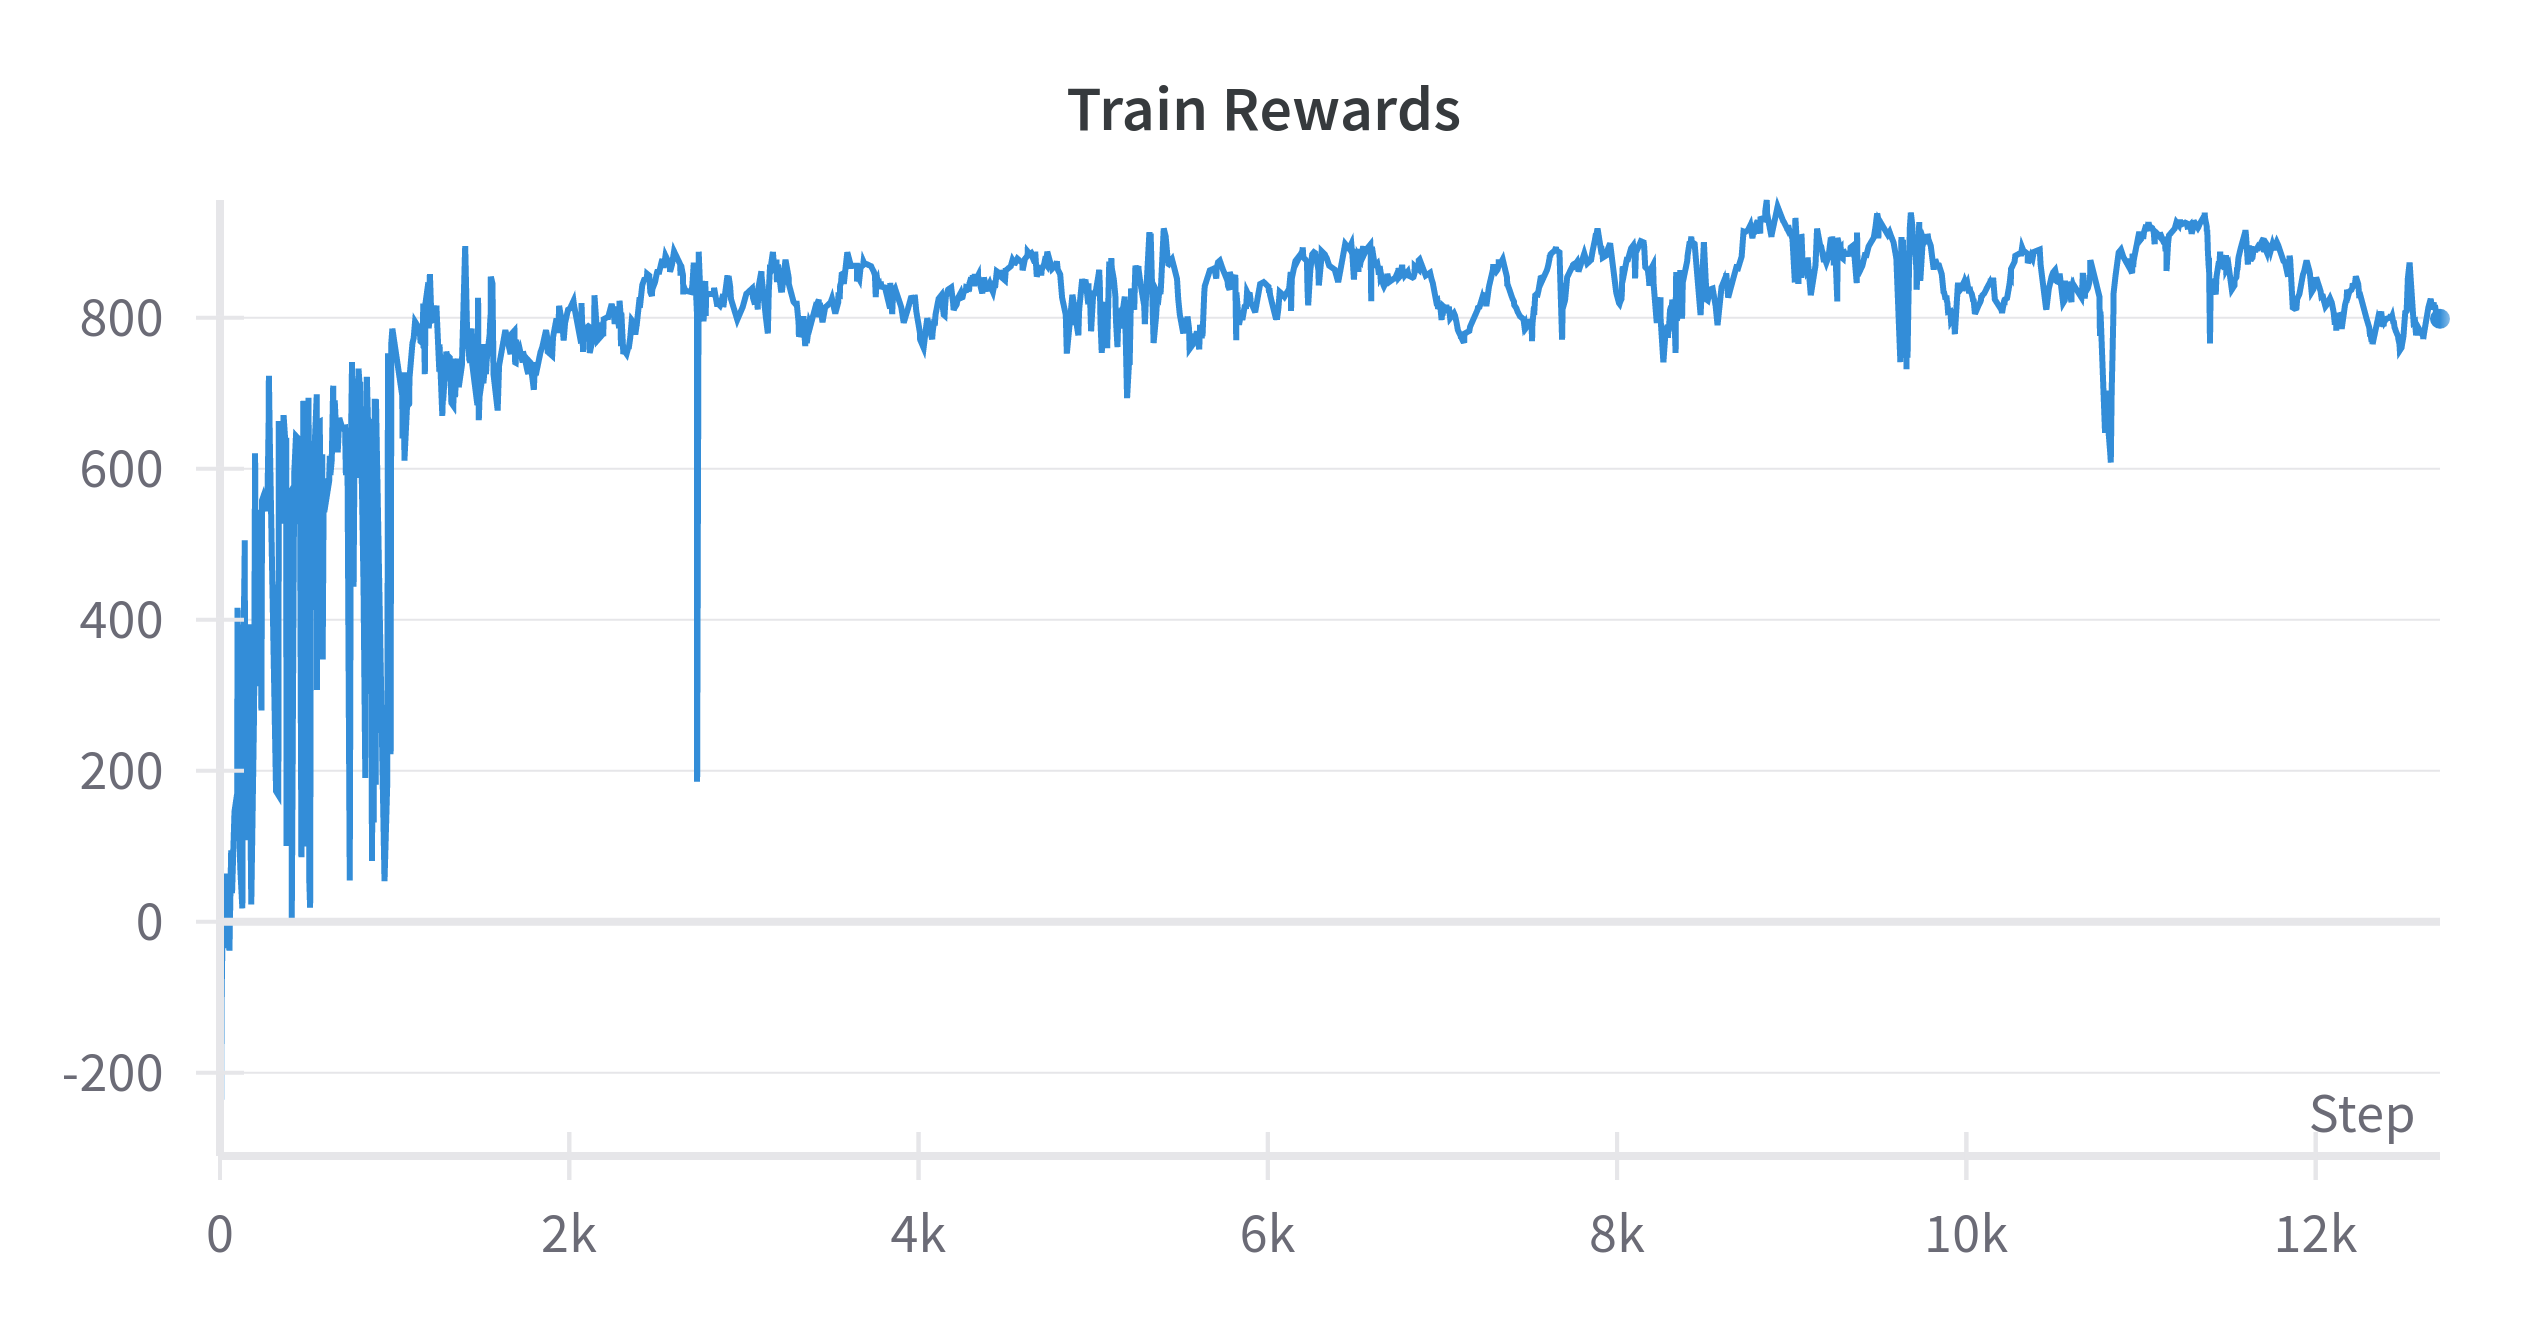
\includegraphics[width=13cm]{reinforce_ant_train.png}
    \caption{Training run rewards vor the ant environment.}
    \label{REIN:ant_tra}
\end{figure}


\newpage
\section{SAC}
As a more advanced agent, an SAC agent was implemented to train the ant.
The implementation was based on the Notebook provieded in excersice 7, and \cite{haarnoja2018soft}.
A challenging part of this Agent was to set up the hyperparameters the right way.
In the first expereiments a phenomenon occured, that the $\alpha$ parameter first went down to zero as
expected, but suddendly exploded towards infinity.
This was due to the numeric log probabilites of the action going towards infinity when the standard deviations
in the gaussian policies are to small.
The problem has been solved by changing the parameter initailization for the actor network and increasing the minimal
standard deviation in the policy.
With similar training lengths as with the REINFORCE agent, the SAC agent achieves much better results.
Since SAC is a off policy learner, the agent can take much more training steps with the same amount of environment steps.
The latter turned out to be the biggest bottleneck.
However the results are not as good as the ones provided by \cite{haarnoja2018soft}.

\begin{figure}
    \centering
    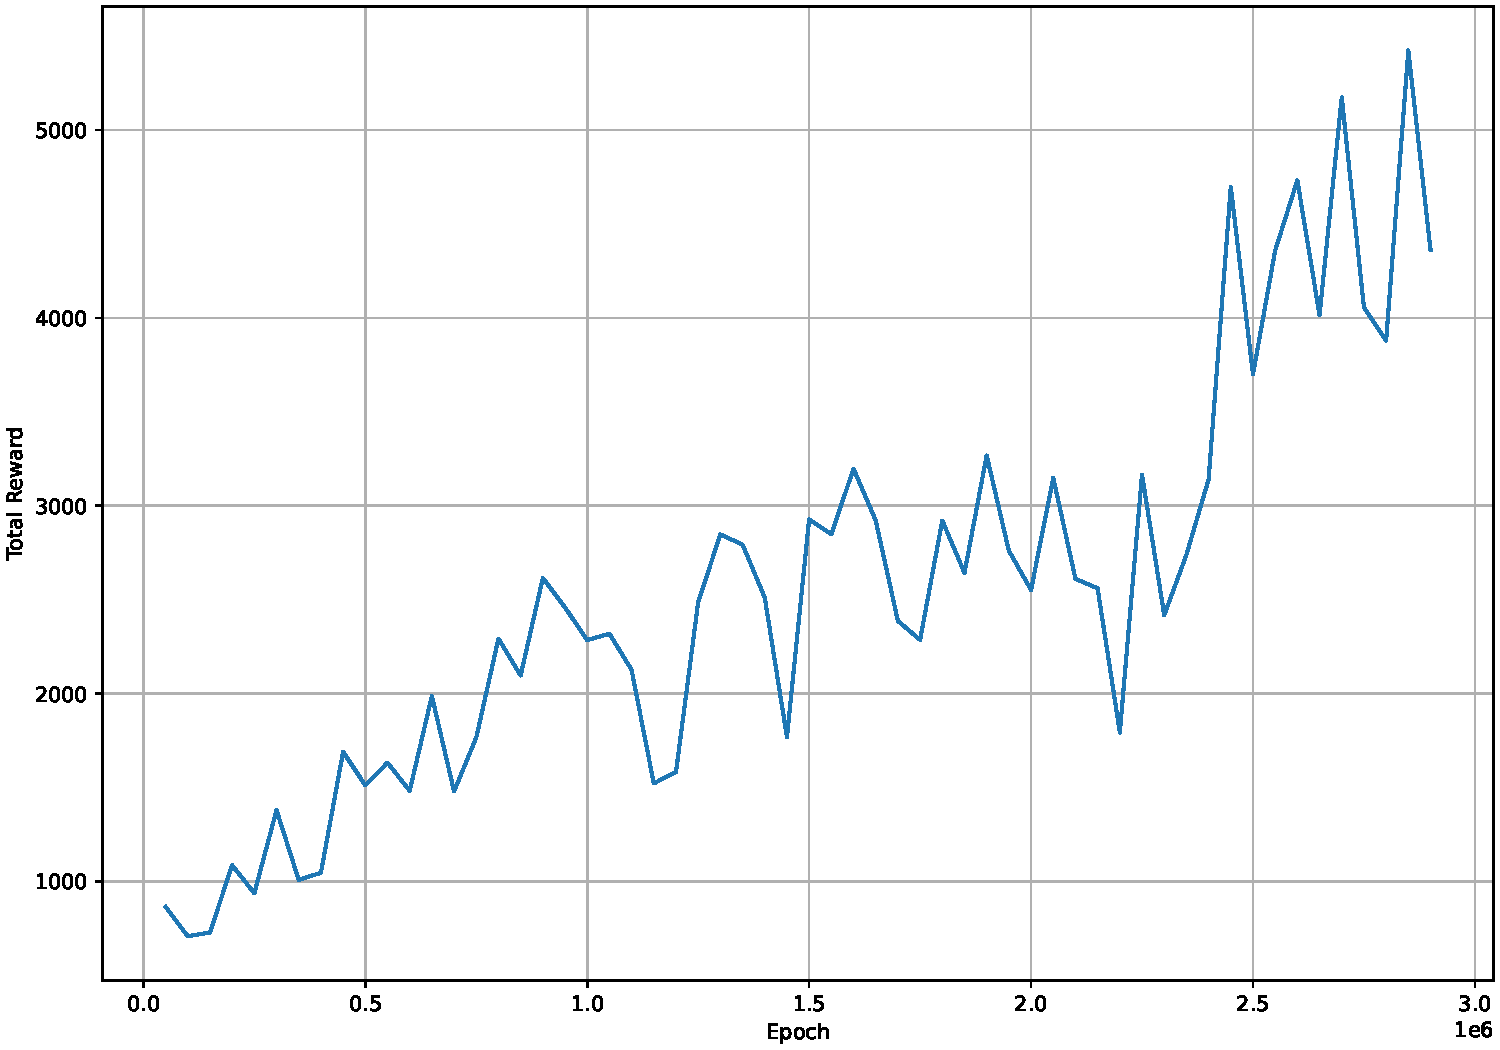
\includegraphics[width=15cm]{test.pdf}
    \caption{Training run rewards vor the ant environment.}
    \label{SAC:test}
\end{figure}

\begin{figure}
    \centering
    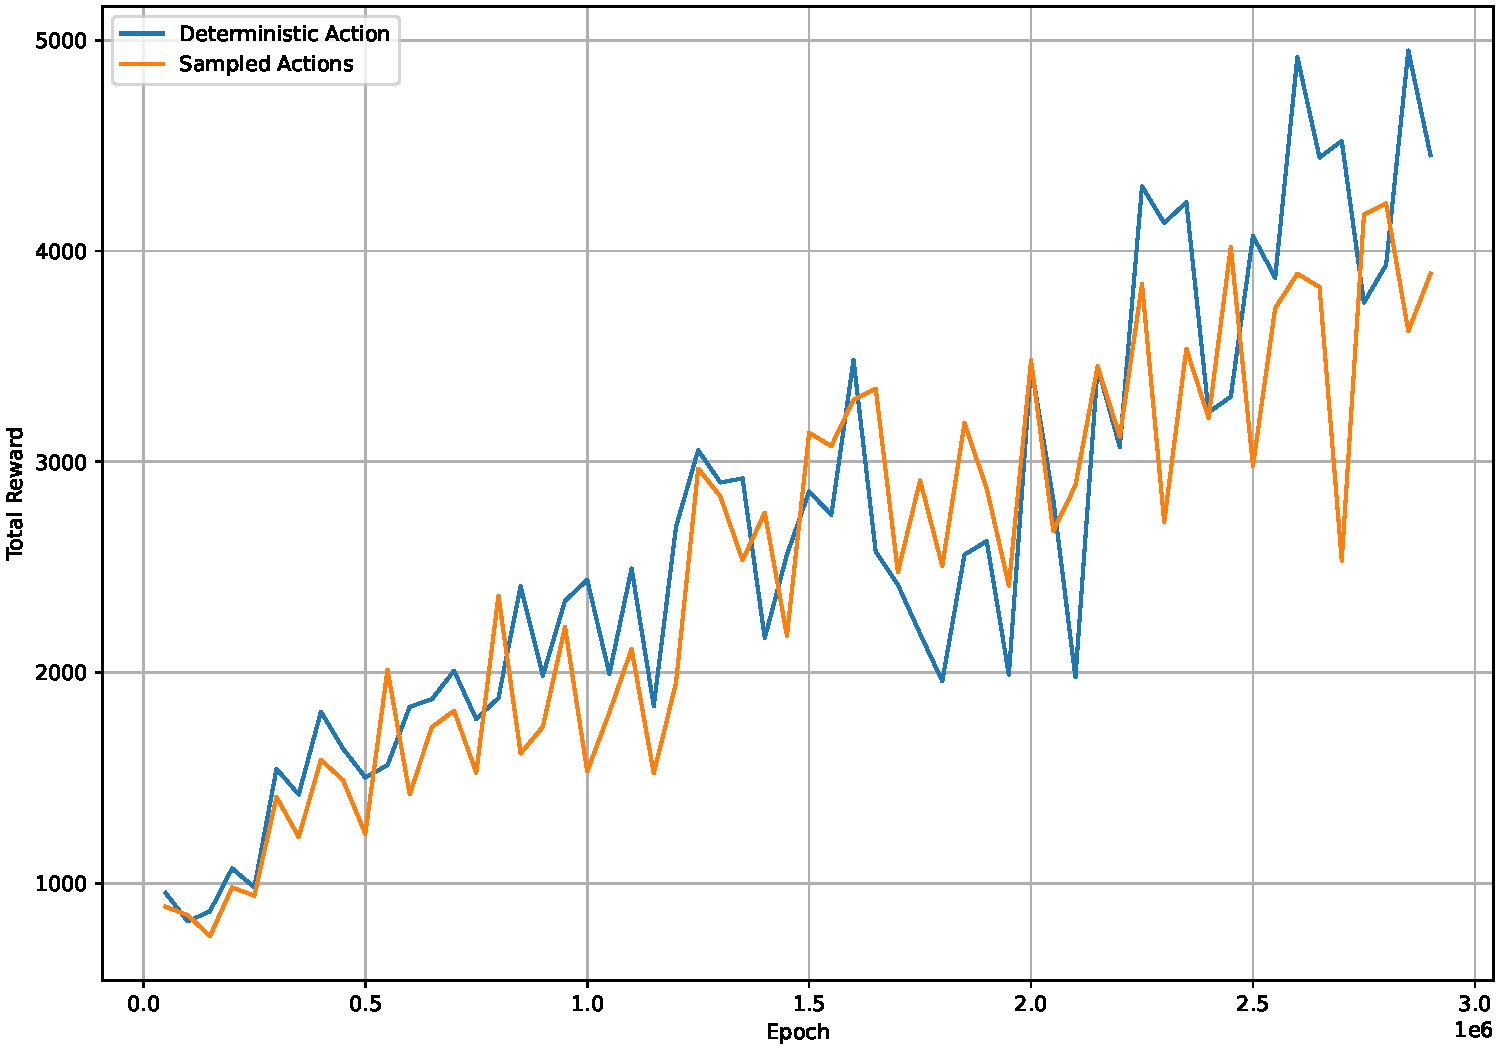
\includegraphics[width=15cm]{stoc_det.pdf}
    \caption{Training run rewards vor the ant environment.}
    \label{SAC:test1}
\end{figure}

\newpage
\section{SAC}
As a more advanced agent, an SAC agent was implemented to train the ant.
The implementation was based on the Notebook provieded in excersice 7, and \cite{haarnoja2018soft} with
the automated entropy adjustement form \cite{haarnoja2019soft}.
A challenging part of this Agent was to set up the hyperparameters the right way.
In the first expereiments a phenomenon occured, that the $\alpha$ parameter first went down to zero as
expected, but suddendly exploded towards infinity.
This was due to the numeric log probabilites of the action going towards infinity when the standard deviations
in the gaussian policies are to small.
The problem has been solved by changing the parameter initailization for the actor network and increasing the minimal
standard deviation in the policy.
With similar training lengths as with the REINFORCE agent, the SAC agent achieves much better results.
Since SAC is a off policy learner, the agent can take much more training steps with the same amount of environment steps.
The latter turned out to be the biggest bottleneck.
However the results are not as good as the ones provided by \cite{haarnoja2018soft}.
Several trainings with different settings were made.
The SAC seemed to be quite robust against minor chnages in the hyperparameters.
Also the outcome was similar whether the loss is based on the learned Q-function or
is an advantage consitsing of the learned Q and Value function.
However one training run stood out and it was the one with the least initial random steps.
Either it was luck or the initial random steps may be a hyperparameter worth finetuning.
Due to the lengths of the trainings this idea could not be further investigated before submission.

\begin{figure}
    \centering
    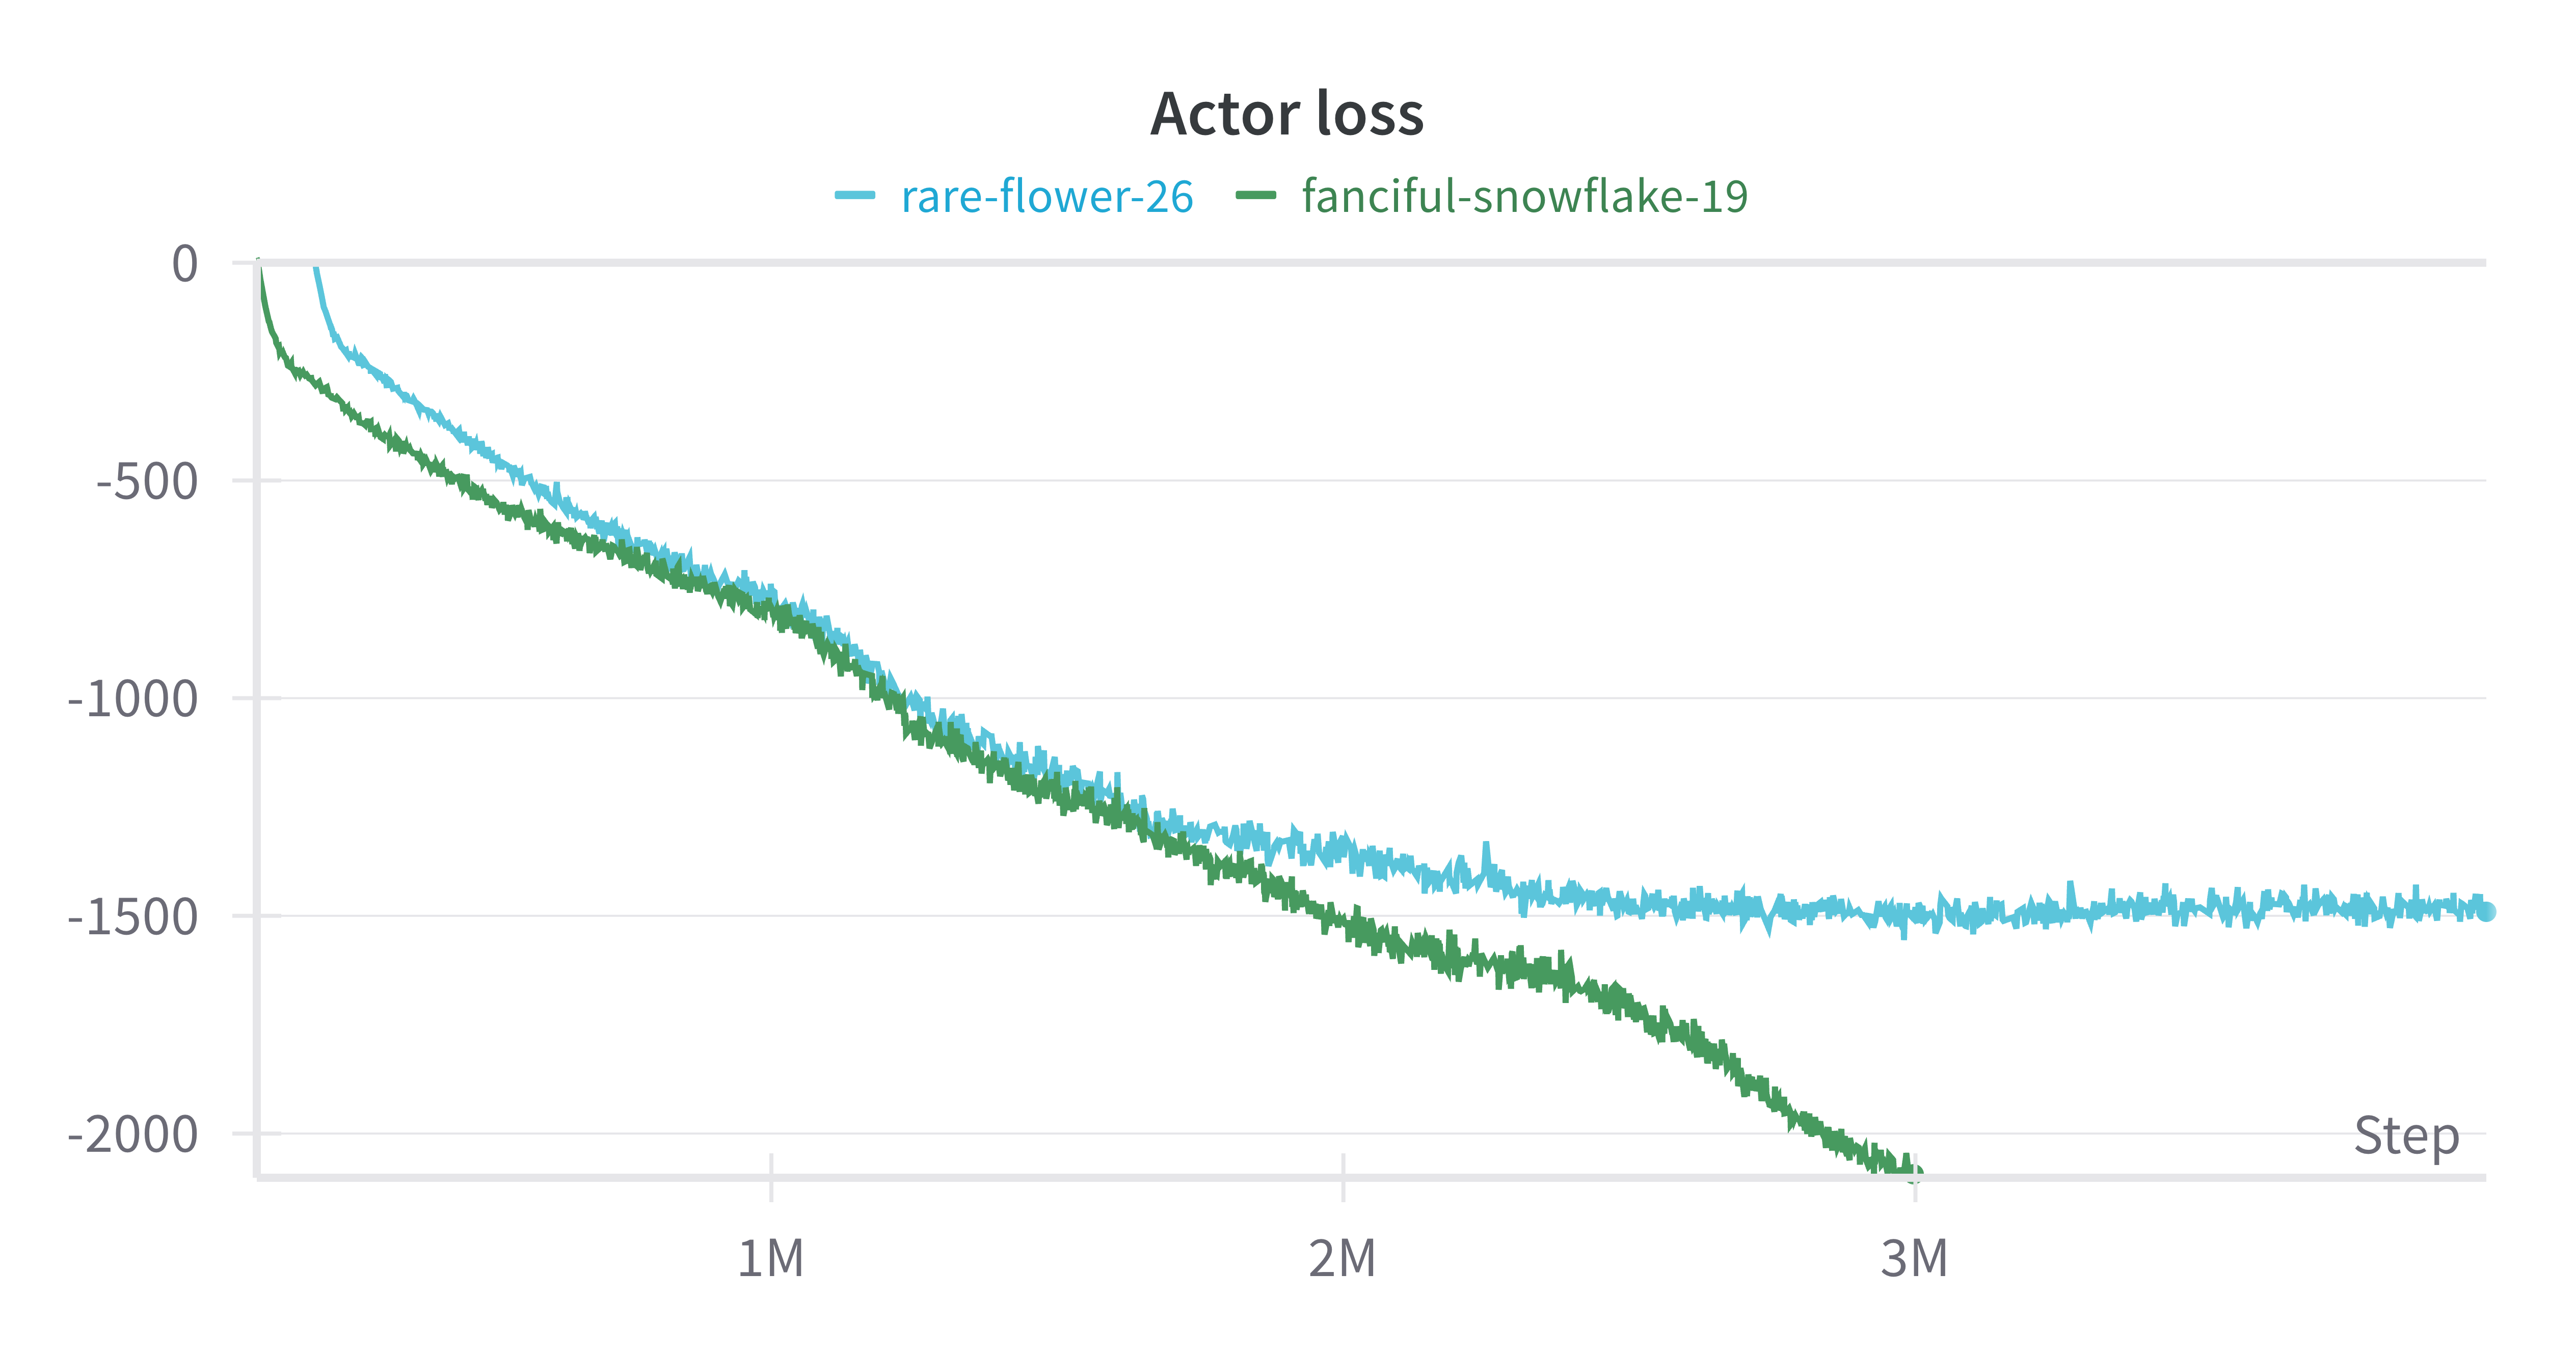
\includegraphics[width=15cm]{SAC_actor_loss.png}
    \caption{Actor loss, in green is the run with 100'000 initial random steps
    and in blue the run with 200'000 inital random steps.}
    \label{SAC:acc_loss}
\end{figure}

\begin{figure}
    \centering
    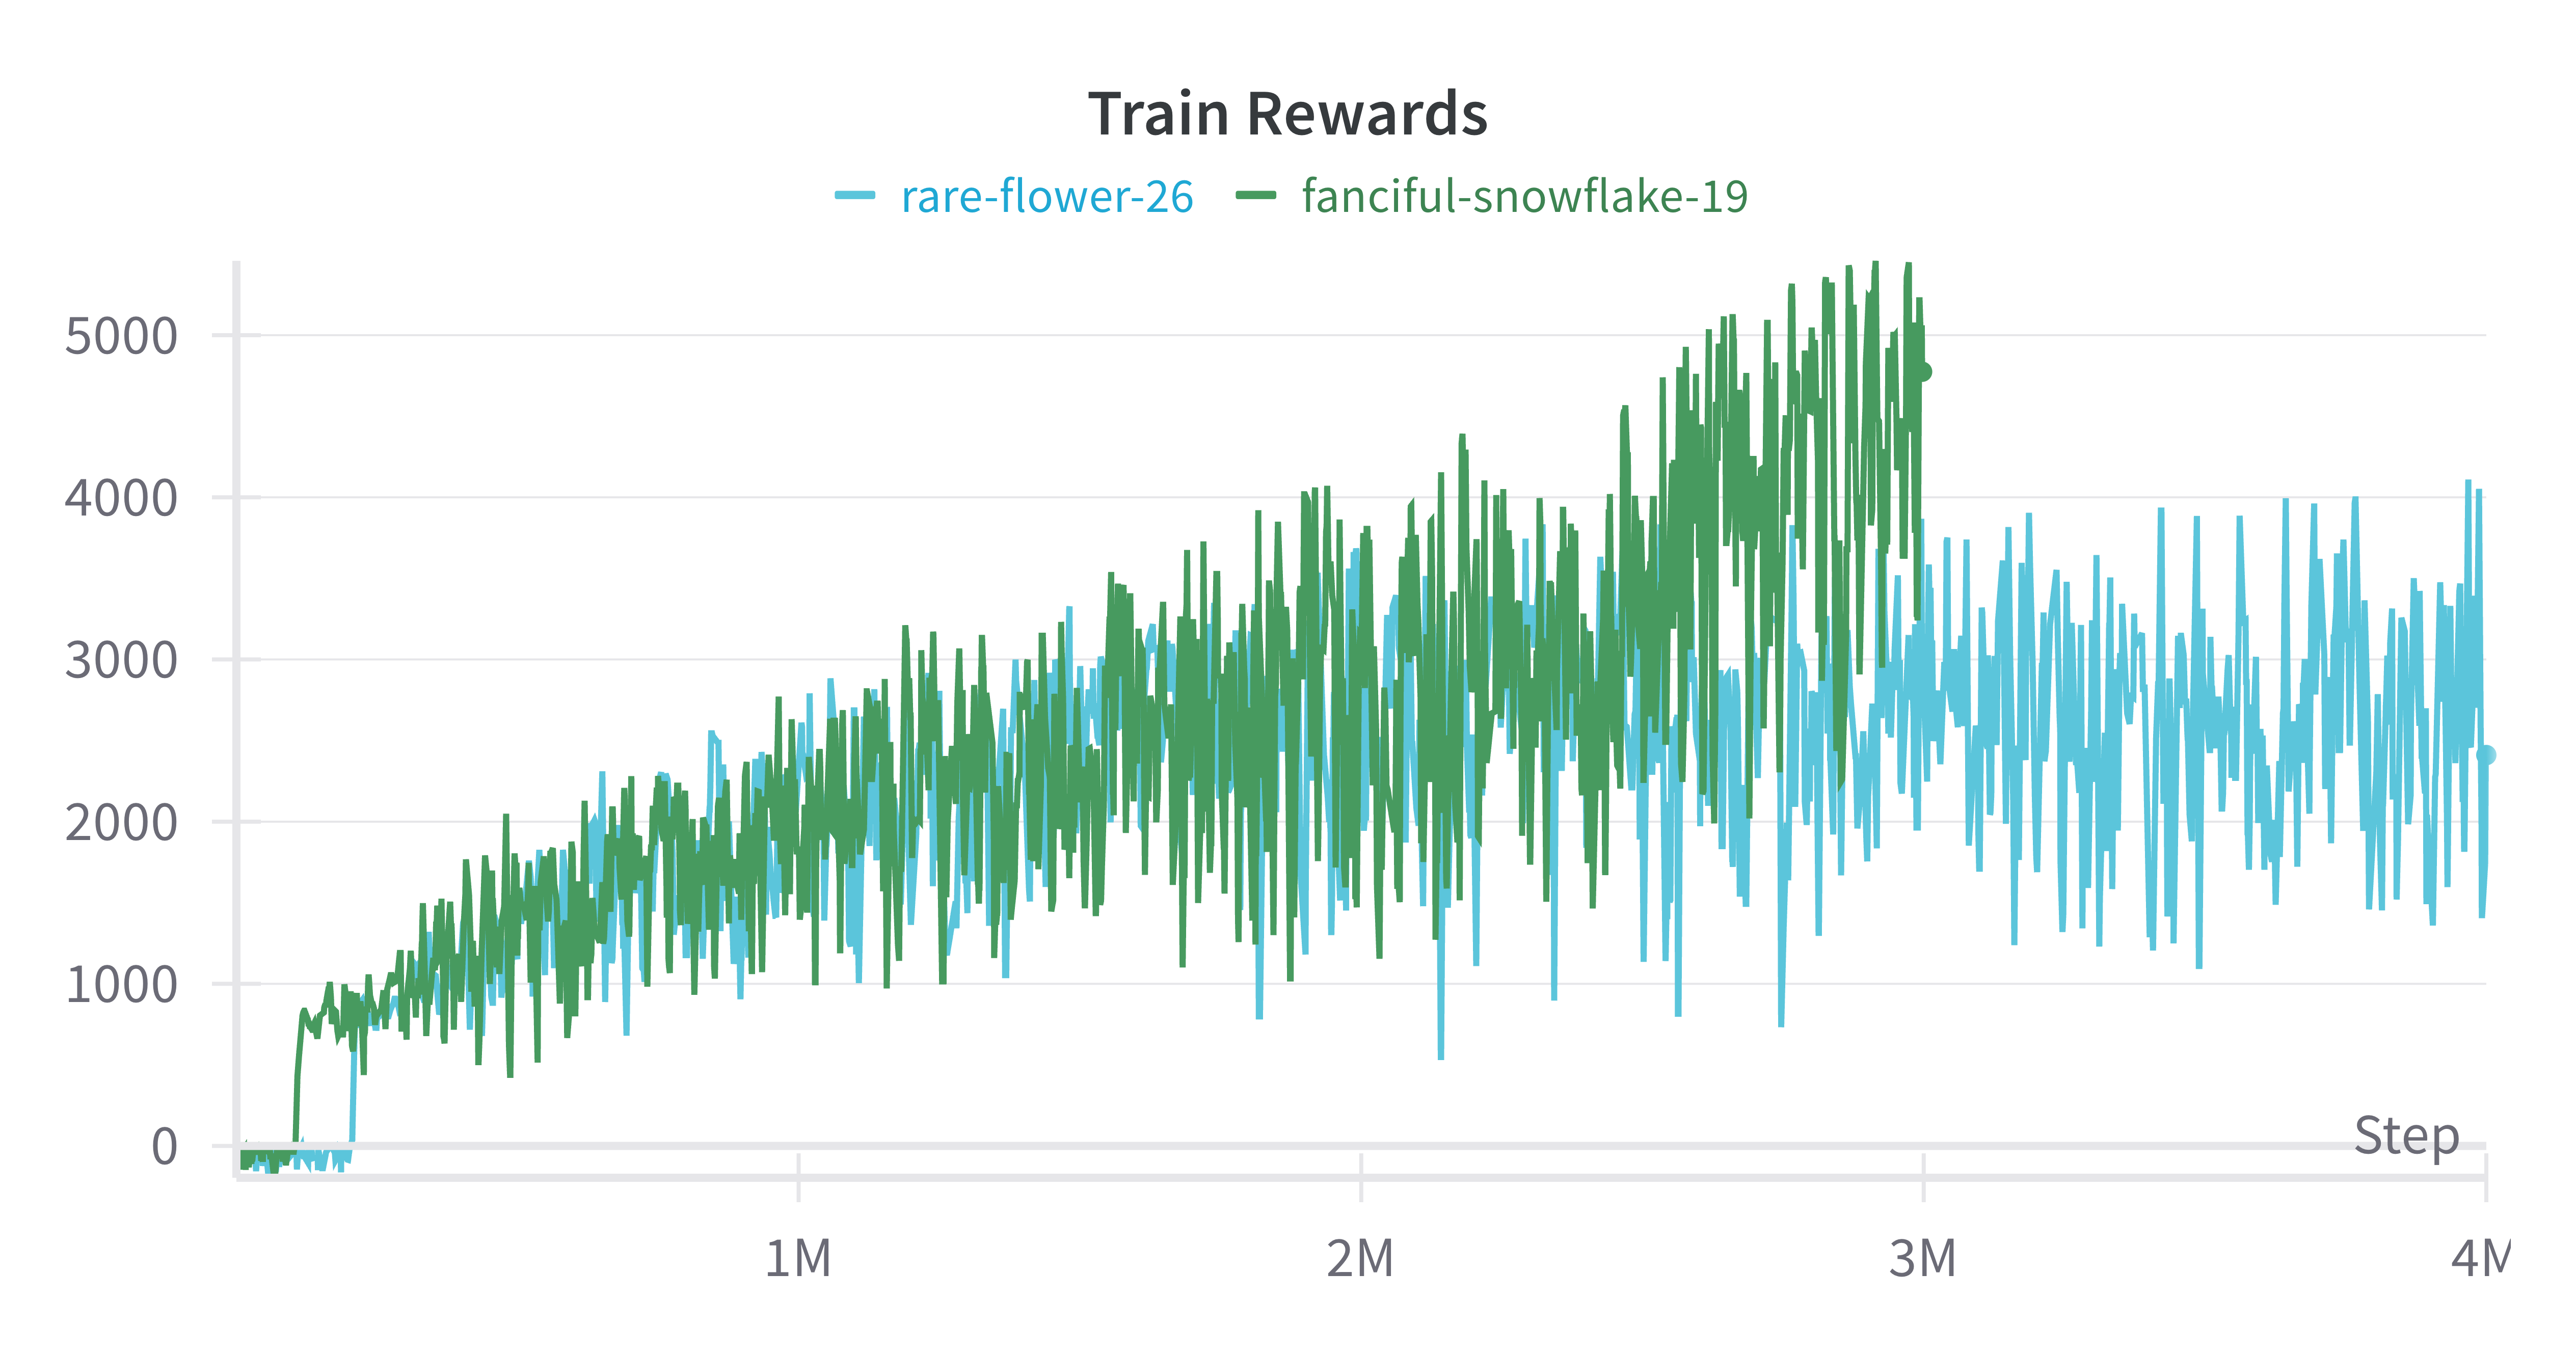
\includegraphics[width=15cm]{SAC_train_reward.png}
    \caption{Training environments rewards, in green is the run with 100'000 initial random steps
    and in blue the run with 200'000 inital random steps.}
    \label{SAC:tr_rew}
\end{figure}

\bibliography{mybib}{}
\bibliographystyle{plain}

\end{document}

\bibliography{mybib}{}
\bibliographystyle{plain}

\end{document}
